
\chapter{Experiments} % Main chapter title





The approaches are trained on dataset "synthetic-50-5" as mentioned in Chapter \ref{ch:04} with 3000 scenes. The screen size is $ 128\times 128 $ in height and width. The corresponding vertex matrix has dimension $ 128\times 128\times3 $, light map has dimension $ 128\times 128 \times 3 $, image has dimension $ 128\times 128 \times 1 $.  The training pipeline use batch size $ 8 $,  Adam optimizer (\cite{adam}), learning rate of  $ 1\times10^{-3} $, learning schedule [8,1000], learning decay factor 0.5. 
The model is trained with PyTorch 1.10.0a0, CUDA 11.4.1, GPU with single NVIDIA GEFORCE RTX 3090. 


\section{GCNN model evaluation}
The GCNN model is the base model of the whole thesis. The architecture is described in \ref{sec:gcnn}. We use a single GCNN to estimate the surface normal based on geometry information. It uses vertex map as input to estimate the corresponding tangent surface normal map. 
%% gcnn-eval
\begin{figure}[H]
	\centering
	\begin{subfigure}[b]{0.18\linewidth}
		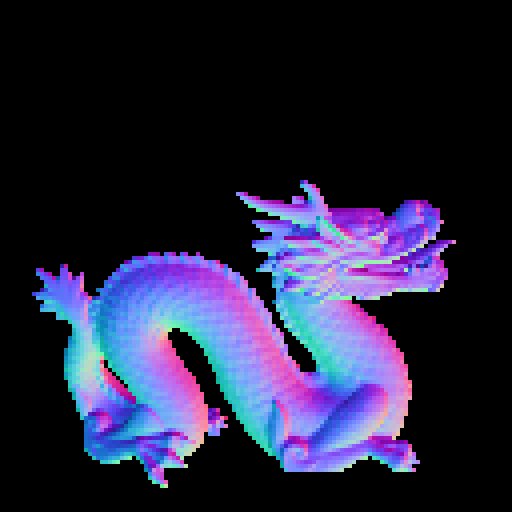
\includegraphics[width=\linewidth]{./Figures/visual_eval/fancy_eval_7_groundtruth.png}
	\end{subfigure}
	\begin{subfigure}[b]{0.18\linewidth}
		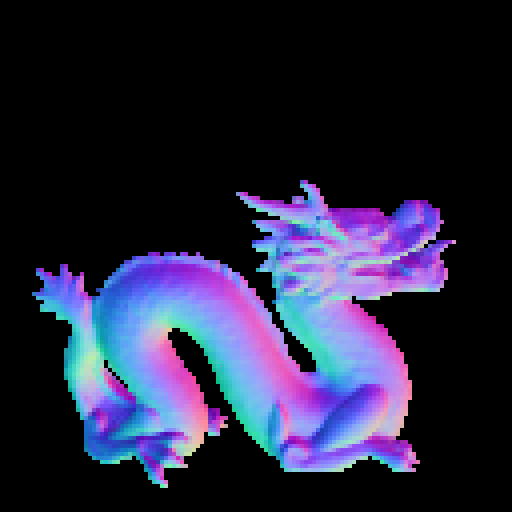
\includegraphics[width=\linewidth]{./Figures/visual_eval/fancy_eval_7_normal_GCNN-GCNN.png}
	\end{subfigure}
	\begin{subfigure}[b]{0.18\linewidth}
		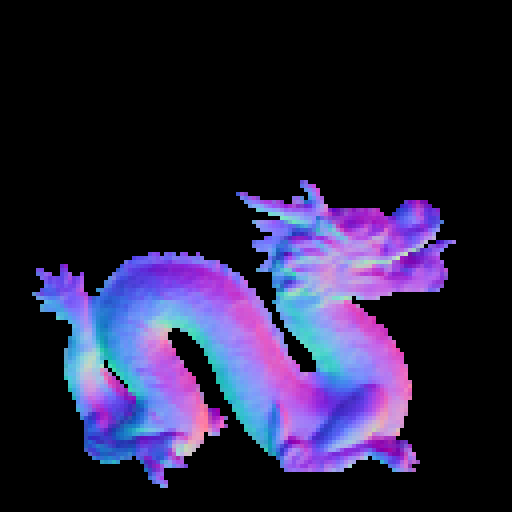
\includegraphics[width=\linewidth]{./Figures/visual_eval/fancy_eval_7_normal_GCNN-CNN.png}
	\end{subfigure}
	\begin{subfigure}[b]{0.18\linewidth}
		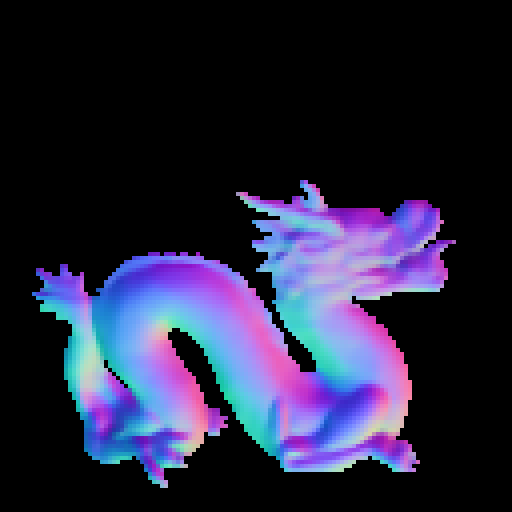
\includegraphics[width=\linewidth]{./Figures/visual_eval/fancy_eval_7_normal_GCNN-NOC.png}
	\end{subfigure}
	\begin{subfigure}[b]{0.18\linewidth}
		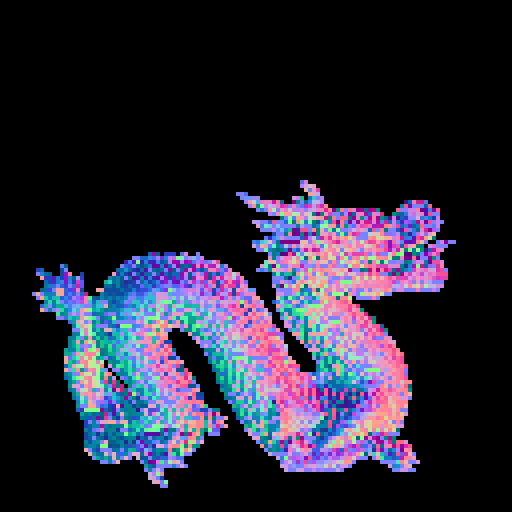
\includegraphics[width=\linewidth]{./Figures/visual_eval/fancy_eval_7_normal_SVD.png}
	\end{subfigure}
	
	\begin{subfigure}[b]{0.18\linewidth}
		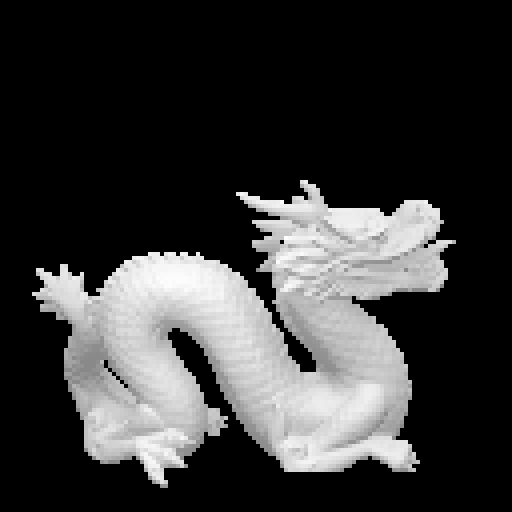
\includegraphics[width=\linewidth]{./Figures/visual_eval/fancy_eval_7_img.png}
		\caption{GT}
	\end{subfigure}
	\begin{subfigure}[b]{0.18\linewidth}
		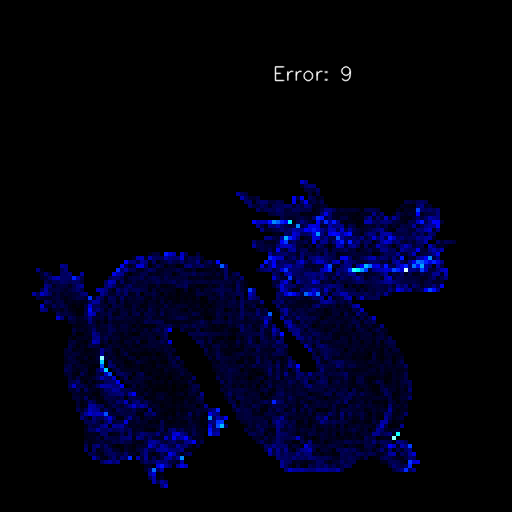
\includegraphics[width=\linewidth]{./Figures/visual_eval/fancy_eval_7_error_GCNN-GCNN.png}
		\caption{GCNN}
	\end{subfigure}
	\begin{subfigure}[b]{0.18\linewidth}
		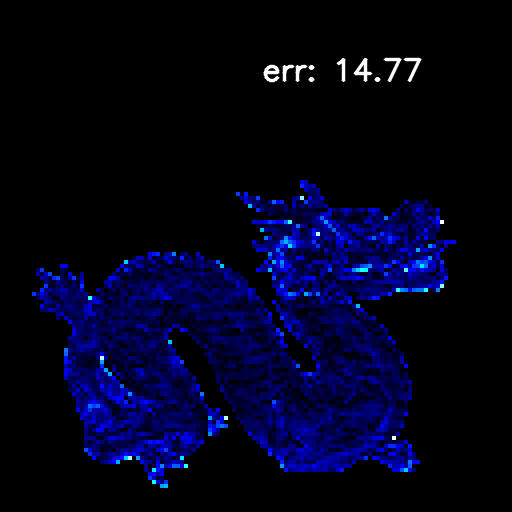
\includegraphics[width=\linewidth]{./Figures/visual_eval/fancy_eval_7_error_GCNN-CNN.png}
		\caption{CNN}
	\end{subfigure}
	\begin{subfigure}[b]{0.18\linewidth}
		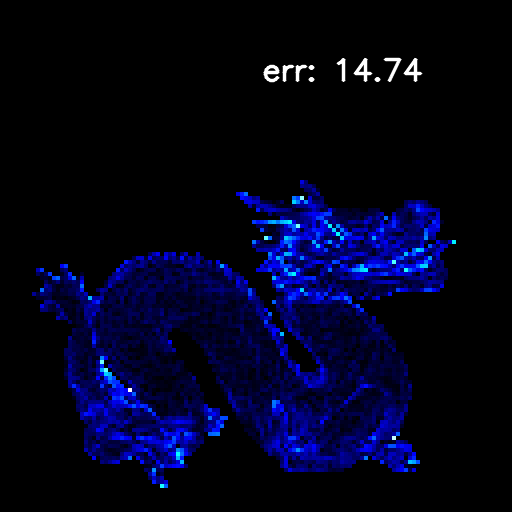
\includegraphics[width=\linewidth]{./Figures/visual_eval/fancy_eval_7_error_GCNN-NOC.png}
		\caption{NOC}
	\end{subfigure}
	\begin{subfigure}[b]{0.18\linewidth}
		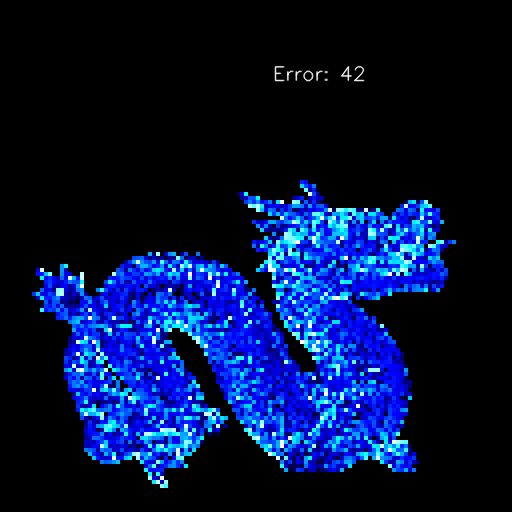
\includegraphics[width=\linewidth]{./Figures/visual_eval/fancy_eval_7_error_SVD.png}
		\caption{SVD}
	\end{subfigure}
	
	\begin{tikzpicture}
		\node[text width=0.1\textwidth] at (10,-1) {90};
		\node[inner sep=0pt] (input) at (8,-1)
		{
\includegraphics[width=.2\textwidth]{./Figures/colorscale_blue.png}};
		\node[text width=0.3\textwidth] at (7,-1) {Error: 0};
	\end{tikzpicture}
	
	\caption{Surface Normal Inference based GCNN model on "Dragon´´ object. The first row shows the estimated surface normal. The second row is the angle error map.}
	\label{fig:gcnn-eval}
\end{figure}


A qualitative evaluation on object "dragon" is shown in Figure \ref{fig:gcnn-eval}. SVD approach is considered as the baseline shown in last column. As shown in the figure, learning based methods performs better than SVD in terms of angle error. The SVD approach is failed to deal with semi-dense input since there exists many points that missing neighbors. The GCNN model is especially good at noise input due to the gated convolution layer design. As a further detailed comparison, \ref{fig:gcnn-eval-synthetic-zoom-in} gives a closer visualization on the same object. 



%% fig:gcnn-eval-synthetic-zoom-in
\begin{figure}[H]
	\centering
	\begin{subfigure}[b]{0.18\linewidth}
		\includegraphics[width=\linewidth]{./Figures/visual_eval/eval_7_normal_GT.png}
	\end{subfigure}
	\begin{subfigure}[b]{0.18\linewidth}
		\includegraphics[width=\linewidth]{./Figures/visual_eval/eval_7_normal_GCNN-GCNN.png}
	\end{subfigure}
	\begin{subfigure}[b]{0.18\linewidth}
		\includegraphics[width=\linewidth]{./Figures/visual_eval/eval_7_normal_GCNN-NOC.png}
	\end{subfigure}
	\begin{subfigure}[b]{0.18\linewidth}
		\includegraphics[width=\linewidth]{./Figures/visual_eval/eval_7_normal_GCNN-CNN.png}
	\end{subfigure}
	\begin{subfigure}[b]{0.18\linewidth}
		\includegraphics[width=\linewidth]{./Figures/visual_eval/eval_7_normal_SVD.png}
	\end{subfigure}
	
	\begin{subfigure}[b]{0.18\linewidth}
		\includegraphics[width=\linewidth]{./Figures/visual_eval/eval_7_img.png}
		\caption{GT}
	\end{subfigure}
	\begin{subfigure}[b]{0.18\linewidth}
		\includegraphics[width=\linewidth]{./Figures/visual_eval/eval_7_error_GCNN-GCNN.png}
		\caption{GCNN}
	\end{subfigure}
	\begin{subfigure}[b]{0.18\linewidth}
		\includegraphics[width=\linewidth]{./Figures/visual_eval/eval_7_error_GCNN-NOC.png}
		\caption{NOC}
	\end{subfigure}
	\begin{subfigure}[b]{0.18\linewidth}
		\includegraphics[width=\linewidth]{./Figures/visual_eval/eval_7_error_GCNN-CNN.png}
		\caption{CNN}
	\end{subfigure}
	\begin{subfigure}[b]{0.18\linewidth}
		\includegraphics[width=\linewidth]{./Figures/visual_eval/eval_7_error_SVD.png}
		\caption{SVD}
	\end{subfigure}
	
	\caption{Zoom in of the center region of Dragon object. The first row is surface normal, the second row is the corresponding errors. NOC model has no skip connnection, CNN model replace gated convolution layer to standard convolution layer.}
	\label{fig:gcnn-eval-synthetic-zoom-in}
\end{figure}
As shown in figure \ref{fig:gcnn-eval-synthetic-zoom-in}, the GCNN method gives a sharper edge prediction on the horn area of the dragon object, as well as the scales, whereas the no skip version (NOC) is blurry in the same area.

The CNN version has the skip connection thus gives a better detail than NOC model. However, if we compare the error map of GCNN and CNN in figure \ref{fig:gcnn-eval}, the CNN has less accurate in the smooth area than GCNN model. Like the dragon body, CNN model has a overall higher error than GCNN. It is because the noise of the input still disturb the CNN model and it takes the input noise into account for normal estimation which deviate to the correct surface normal. When we look back to the GCNN based method, we can found that the surface normal has better performance in the smooth area compare to the CNN approach and a sharp detail compare to the no skip connection version.

Table \ref{tab:gcnn-eval} gives a quantitative evaluation for GCNN model. It bases on 100 different test scenes in the "synthetic-50-5´´ dataset with angle metrics for evaluation.



\begin{table}[H]
	
	\centering
	\begin{tabular}{l l l l l l }
		\tabhead{Model} & \tabhead{Angle} & \tabhead{Time /ms} & \tabhead{bz} & \tabhead{lr-schedule} & \tabhead{lr-df}\\
		SVD(baseline)  & 41.14  & 320.40 & 8 & 8,1000 & 0.5\\ 
		\hline
		GCNN  & 10.64  & 10.44 & 8 & 8,1000 & 0.5\\ 
		\hline
		GCNN-NOC & 13.61 & 5.38 & 8 & 8,1000 & 0.5\\
		\hline
		CNN & 15.35 & 4.15 & 8 & 8,1000 & 0.5\\
	\end{tabular}
	\caption{The performance of the GCNN model for geometry information based normal inference. The angle error is the average angle error of all valid pixels in the test case. bz stands for batch size, lr-schedule stands for learning rate schedule, lr-df stands for learning rate decay factor.}	
	\label{tab:gcnn-eval}
\end{table}





\newpage
\section{Surface Normal Inference based on Calibrated Illuminated RGBD images }

For the approach using illuminated calibrated RGBD image, the task is undertaken by Trip-Net introduced in \ref{sec:trip-net}. 
The qualitative evaluation is shown in figure \ref{fig:trip-eval}. As a comparison, we placed GCNN result in the last column. The training settings for all the models are exact the same to ensure fairness. As shown in the figure, TripNet uses illuminated calibrated RGBD image has a better performance than GCNN model. The dragon scales are sharper in TripNet result. Figure \ref{fig:tripnet-eval-synthetic-zoom-in} gives a closer visualization.
%% TripNet-eval
\begin{figure}[H]
	\centering
	\begin{subfigure}[b]{0.18\linewidth}
		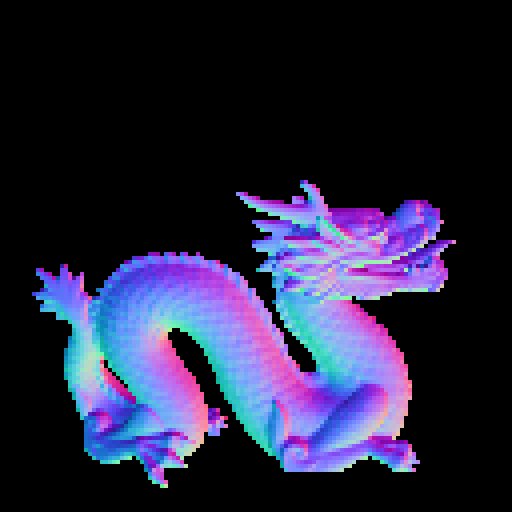
\includegraphics[width=\linewidth]{./Figures/visual_eval/fancy_eval_7_groundtruth.png}
	\end{subfigure}
	\begin{subfigure}[b]{0.18\linewidth}
		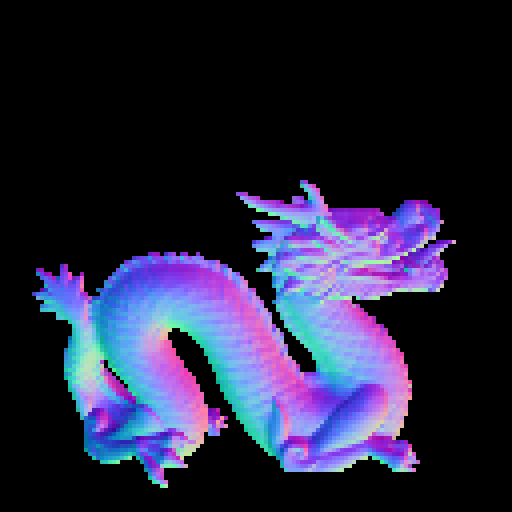
\includegraphics[width=\linewidth]{./Figures/visual_eval/fancy_eval_7_normal_an2-8-1000.png}
	\end{subfigure}
	\begin{subfigure}[b]{0.18\linewidth}
		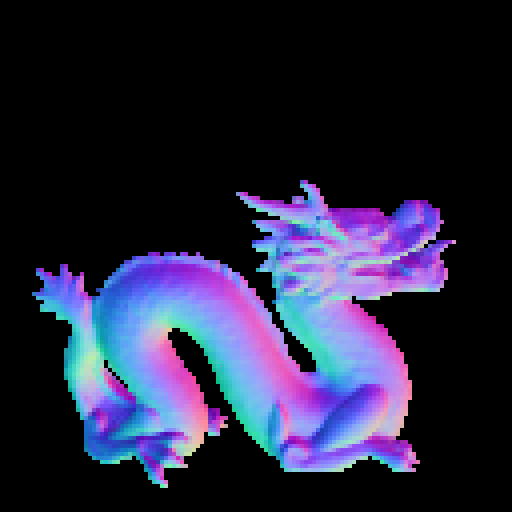
\includegraphics[width=\linewidth]{./Figures/visual_eval/fancy_eval_7_normal_GCNN-GCNN.png}
	\end{subfigure}
	
	\begin{subfigure}[b]{0.18\linewidth}
		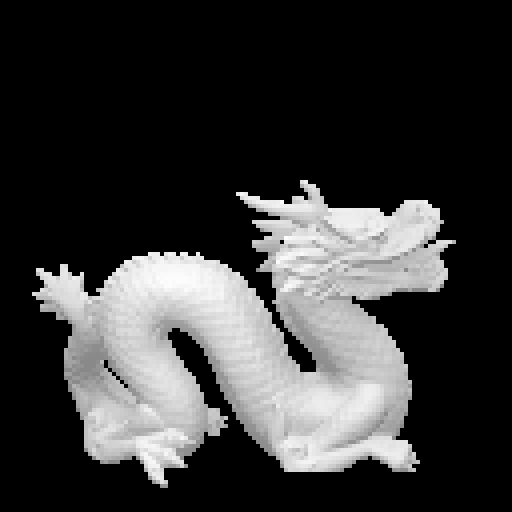
\includegraphics[width=\linewidth]{./Figures/visual_eval/fancy_eval_7_img.png}
		\caption{GT}
	\end{subfigure}
	\begin{subfigure}[b]{0.18\linewidth}
		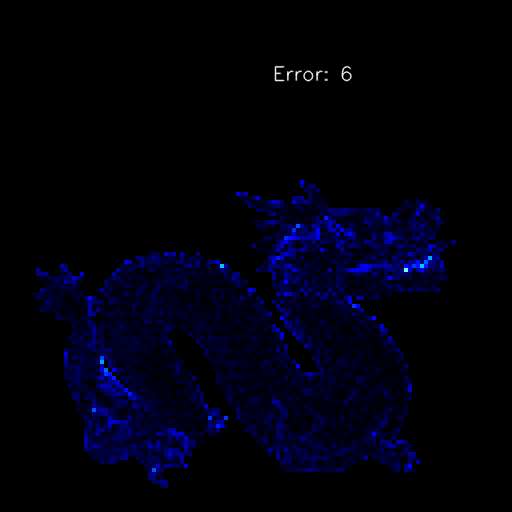
\includegraphics[width=\linewidth]{./Figures/visual_eval/fancy_eval_7_error_an2-8-1000.png}
		\caption{TripNet}
	\end{subfigure}
	\begin{subfigure}[b]{0.18\linewidth}
		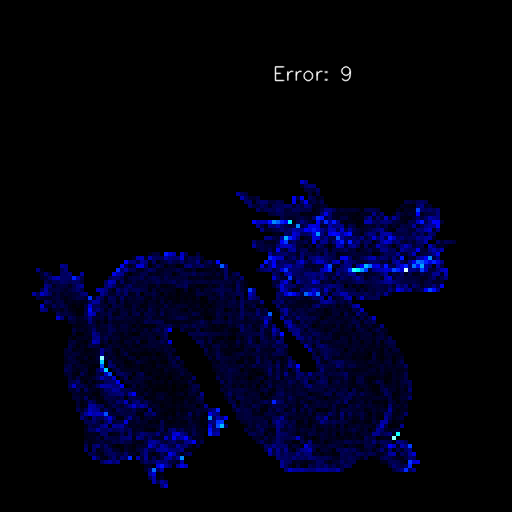
\includegraphics[width=\linewidth]{./Figures/visual_eval/fancy_eval_7_error_GCNN-GCNN.png}
		\caption{GCNN}
	\end{subfigure}
	
	
	\begin{tikzpicture}
		\node[text width=0.1\textwidth] at (10,-1) {90};
		\node[inner sep=0pt] (input) at (8,-1)
		{
\includegraphics[width=.2\textwidth]{./Figures/colorscale_blue.png}};
		\node[text width=0.3\textwidth] at (7,-1) {Error: 0};
	\end{tikzpicture}
	
	\caption{TripNet qualitative evaluation. Surface Normal Inference on ``Dragon" object. The first row shows the estimated surface normal. The second row is the angle error map.}
	\label{fig:trip-eval}
\end{figure}

%% tripNet zoom in eval
\begin{figure}[H]
	\centering
	\begin{subfigure}[b]{0.18\linewidth}
		\includegraphics[width=\linewidth]{./Figures/visual_eval/eval_7_normal_GT.png}
	\end{subfigure}
	\begin{subfigure}[b]{0.18\linewidth}
		\includegraphics[width=\linewidth]{./Figures/visual_eval/eval_7_normal_an2-8-1000.png}
	\end{subfigure}
	\begin{subfigure}[b]{0.18\linewidth}
		\includegraphics[width=\linewidth]{./Figures/visual_eval/eval_7_normal_GCNN-GCNN.png}
	\end{subfigure}
	
	\begin{subfigure}[b]{0.18\linewidth}
		\includegraphics[width=\linewidth]{./Figures/visual_eval/eval_7_img.png}
		\caption{GT}
	\end{subfigure}
	\begin{subfigure}[b]{0.18\linewidth}
		\includegraphics[width=\linewidth]{./Figures/visual_eval/eval_7_error_an2-8-1000.png}
		\caption{Trip-Net}
	\end{subfigure}
	\begin{subfigure}[b]{0.18\linewidth}
		\includegraphics[width=\linewidth]{./Figures/visual_eval/eval_7_error_GCNN-GCNN.png}
		\caption{GCNN}
	\end{subfigure}
	
	
	\caption{Zoom in of the center region of Dragon object. The first row is surface normal, the second row is the corresponding errors.}
	\label{fig:tripnet-eval-synthetic-zoom-in}
\end{figure}


\begin{table}[th]
	
	\centering
	\begin{tabular}{l l l l l l l }
		\tabhead{Model} & \tabhead{Angle} & \tabhead{Time /ms} & \tabhead{bz} & \tabhead{lr-schedule} & \tabhead{lr-df} & \tabhead{l/i. Nr.}\\
		SVD  & 41.14  & 320.40 & - & - & - & 0 \\ 
		\hline
		GCNN  & 10.64 & 10.44 & 8 & 8,1000 & 0.5 & 0 \\
		\hline
		TripNet-CNN & 10.46 & 28.74 & 8 & 8,1000  & 0.5 & 1 \\
		\hline
		TripNet-F1B & 9.22 &44.59 & 8 & 8,1000  & 0.5 & 1 \\
		\hline
		TripNet & \textbf{9.17} & 43.79 & 8 & 8,1000  & 0.5 & 1 \\
	\end{tabular}
	\caption{A quantitative evaluation on proposed approaches. The angle error is the average angle error of all valid pixels in the test case. The time unit is in millisecond. bz is the batch size, lr-schedule is learning rate schedule. lr-df is learning rate decay factor, l/i. Nr is the number of light-image maps used for each scene}	
	\label{tab:model-error}
\end{table}




\subsection{Comparison}

%% Final-Visual
\begin{figure}[th]
	\centering
	\begin{subfigure}[b]{0.24\linewidth}
		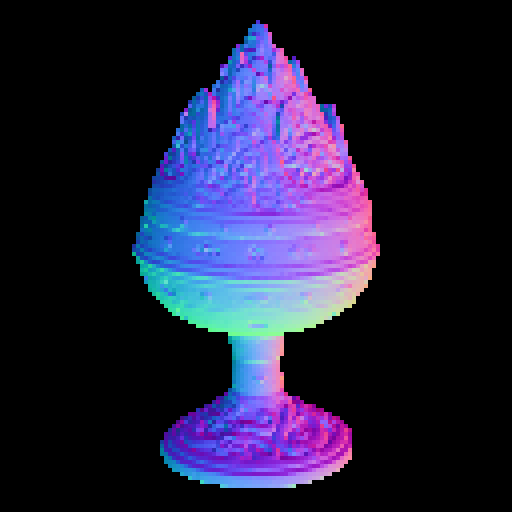
\includegraphics[width=\linewidth]{./Figures/visual_eval/fancy_eval_2_groundtruth.png}
	\end{subfigure}
	\begin{subfigure}[b]{0.24\linewidth}
		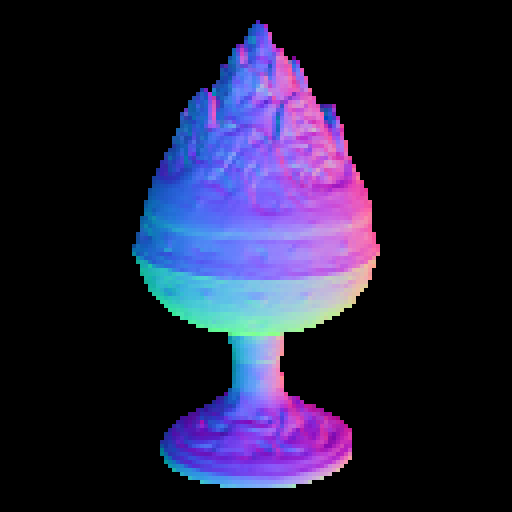
\includegraphics[width=\linewidth]{./Figures/visual_eval/fancy_eval_2_normal_an2-8-1000.png}
	\end{subfigure}
	\begin{subfigure}[b]{0.24\linewidth}
		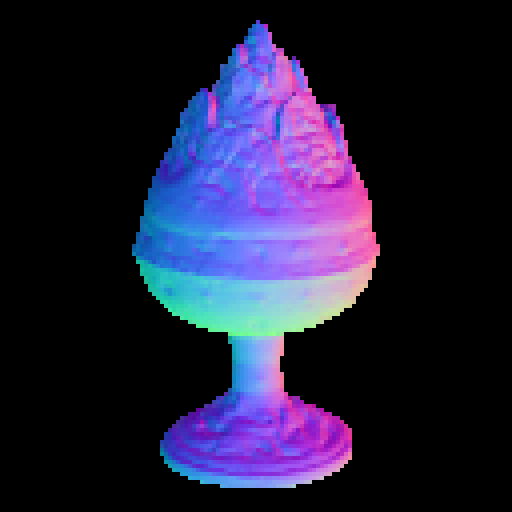
\includegraphics[width=\linewidth]{./Figures/visual_eval/fancy_eval_2_normal_GCNN-GCNN.png}
	\end{subfigure}
	\begin{subfigure}[b]{0.24\linewidth}
		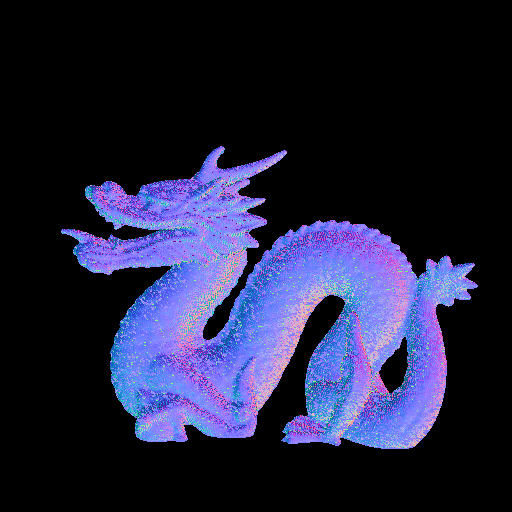
\includegraphics[width=\linewidth]{./Figures/visual_eval/fancy_eval_2_normal_SVD.png}
	\end{subfigure}
	
	\begin{subfigure}[b]{0.24\linewidth}
		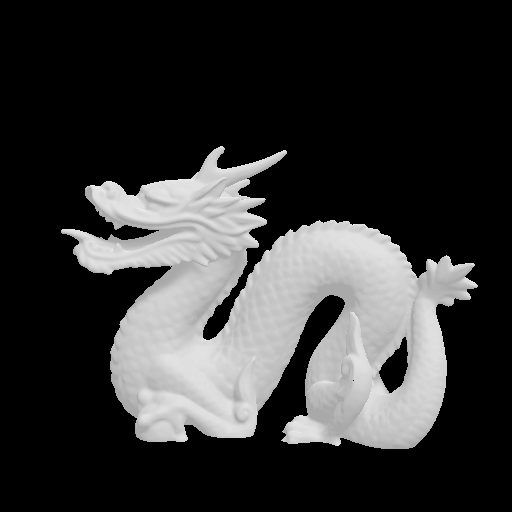
\includegraphics[width=\linewidth]{./Figures/visual_eval/fancy_eval_2_img.png}
	\end{subfigure}
	\begin{subfigure}[b]{0.24\linewidth}
		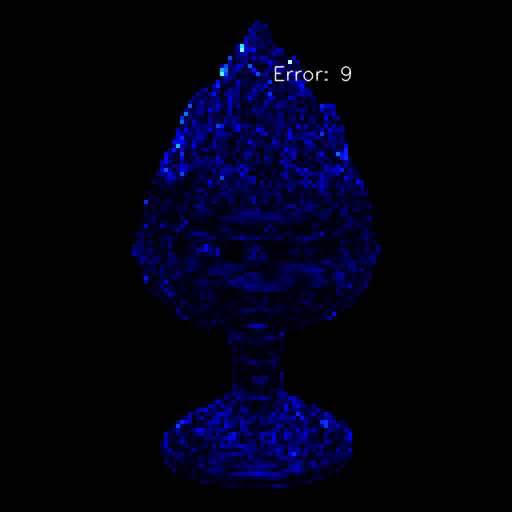
\includegraphics[width=\linewidth]{./Figures/visual_eval/fancy_eval_2_error_an2-8-1000.png}
	\end{subfigure}
	\begin{subfigure}[b]{0.24\linewidth}
		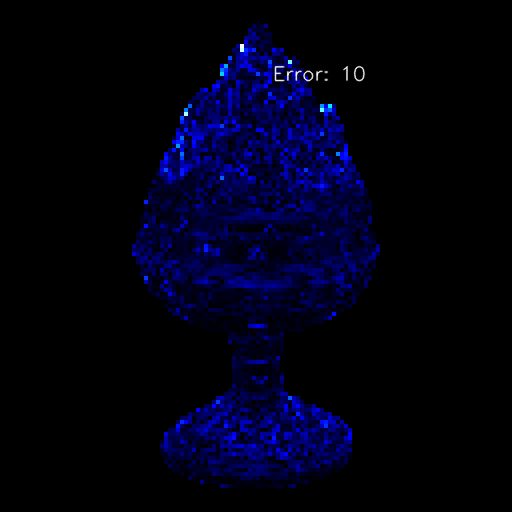
\includegraphics[width=\linewidth]{./Figures/visual_eval/fancy_eval_2_error_GCNN-GCNN.png}
	\end{subfigure}
	\begin{subfigure}[b]{0.24\linewidth}
		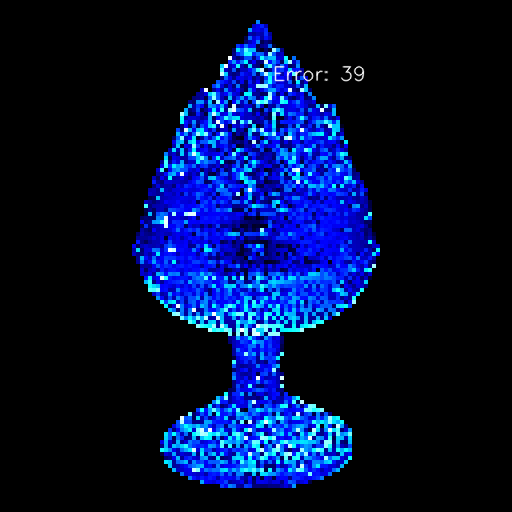
\includegraphics[width=\linewidth]{./Figures/visual_eval/fancy_eval_2_error_SVD.png}
	\end{subfigure}
	
	\begin{subfigure}[b]{0.24\linewidth}
		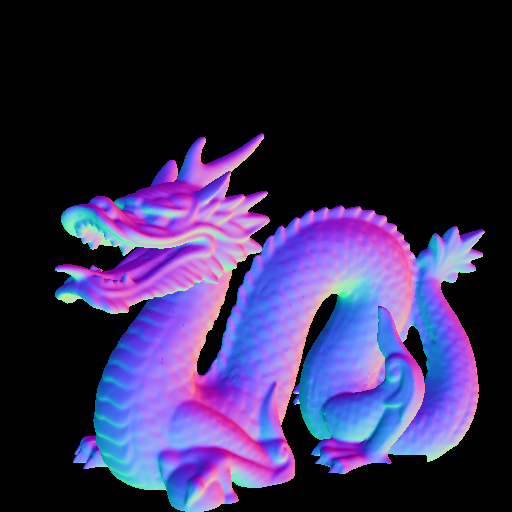
\includegraphics[width=\linewidth]{./Figures/visual_eval/fancy_eval_3_groundtruth.png}
	\end{subfigure}
	\begin{subfigure}[b]{0.24\linewidth}
		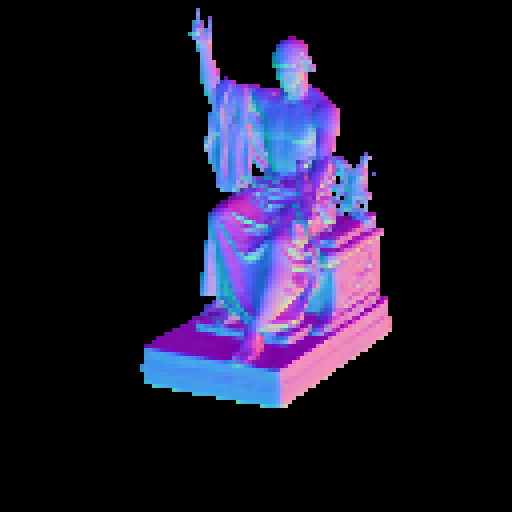
\includegraphics[width=\linewidth]{./Figures/visual_eval/fancy_eval_3_normal_an2-8-1000.png}
	\end{subfigure}
	\begin{subfigure}[b]{0.24\linewidth}
		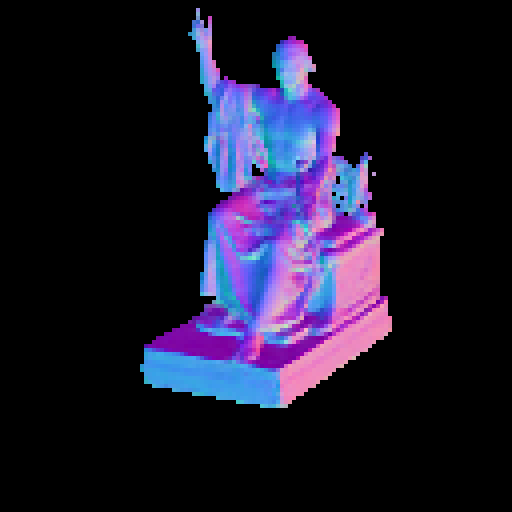
\includegraphics[width=\linewidth]{./Figures/visual_eval/fancy_eval_3_normal_GCNN-GCNN.png}
	\end{subfigure}
	\begin{subfigure}[b]{0.24\linewidth}
		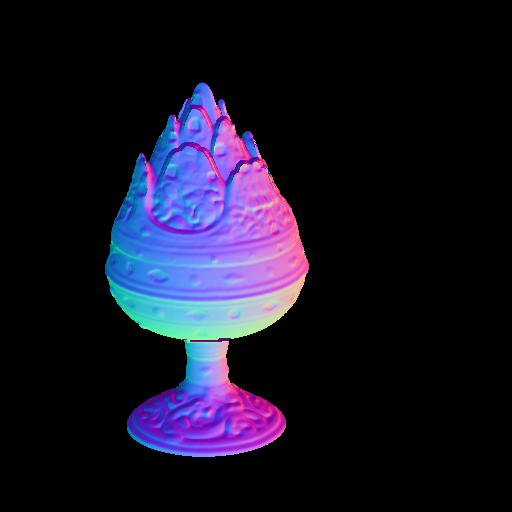
\includegraphics[width=\linewidth]{./Figures/visual_eval/fancy_eval_3_normal_SVD.png}
	\end{subfigure}
	
	
	
	\begin{subfigure}[b]{0.24\linewidth}
		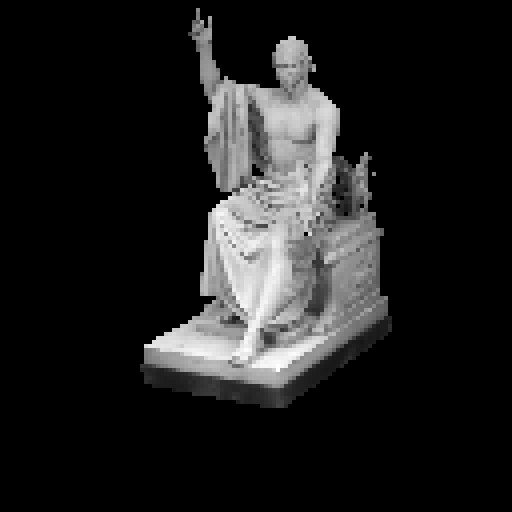
\includegraphics[width=\linewidth]{./Figures/visual_eval/fancy_eval_3_img.png}
	\end{subfigure}
	\begin{subfigure}[b]{0.24\linewidth}
		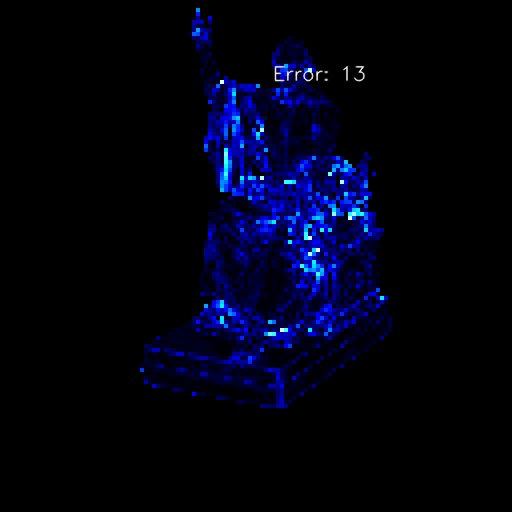
\includegraphics[width=\linewidth]{./Figures/visual_eval/fancy_eval_3_error_an2-8-1000.png}
	\end{subfigure}
	\begin{subfigure}[b]{0.24\linewidth}
		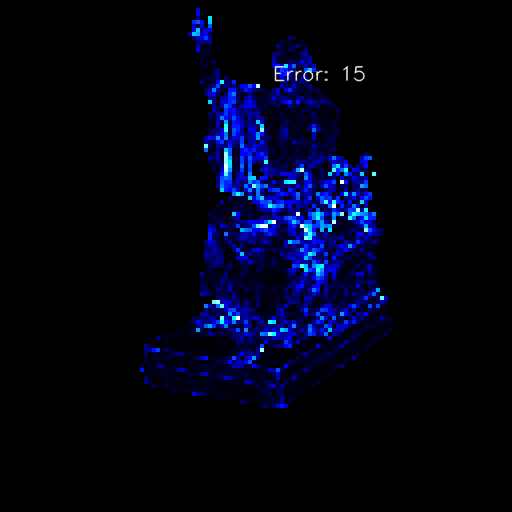
\includegraphics[width=\linewidth]{./Figures/visual_eval/fancy_eval_3_error_GCNN-GCNN.png}
	\end{subfigure}
	\begin{subfigure}[b]{0.24\linewidth}
		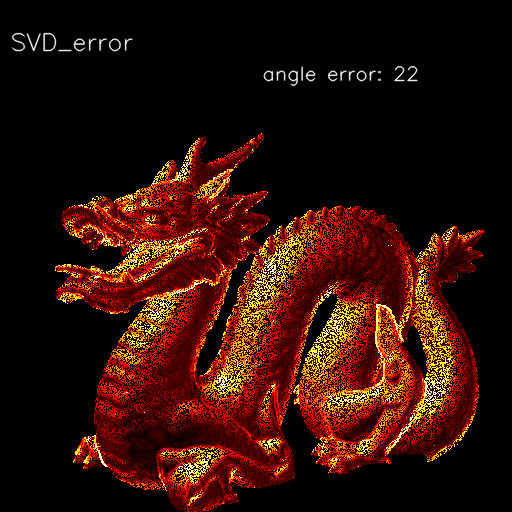
\includegraphics[width=\linewidth]{./Figures/visual_eval/fancy_eval_3_error_SVD.png}
	\end{subfigure}
	
	\begin{subfigure}[b]{0.24\linewidth}
		\includegraphics[width=\linewidth]{./Figures/visual_eval/fancy_eval_9_groundtruth.png}
	\end{subfigure}
	\begin{subfigure}[b]{0.24\linewidth}
		\includegraphics[width=\linewidth]{./Figures/visual_eval/fancy_eval_9_normal_an2-8-1000.png}
	\end{subfigure}
	\begin{subfigure}[b]{0.24\linewidth}
		\includegraphics[width=\linewidth]{./Figures/visual_eval/fancy_eval_9_normal_GCNN-GCNN.png}
	\end{subfigure}
	\begin{subfigure}[b]{0.24\linewidth}
		\includegraphics[width=\linewidth]{./Figures/visual_eval/fancy_eval_9_normal_SVD.png}
	\end{subfigure}
	
	
	\begin{subfigure}[b]{0.24\linewidth}
		\includegraphics[width=\linewidth]{./Figures/visual_eval/fancy_eval_9_img.png}
		\caption{GT}
	\end{subfigure}
	\begin{subfigure}[b]{0.24\linewidth}
		\includegraphics[width=\linewidth]{./Figures/visual_eval/fancy_eval_9_error_an2-8-1000.png}
		\caption{TripNet}
	\end{subfigure}
	\begin{subfigure}[b]{0.24\linewidth}
		\includegraphics[width=\linewidth]{./Figures/visual_eval/fancy_eval_9_error_GCNN-GCNN.png}
		\caption{GCNN}
	\end{subfigure}
	\begin{subfigure}[b]{0.24\linewidth}
		\includegraphics[width=\linewidth]{./Figures/visual_eval/fancy_eval_9_error_SVD.png}
		\caption{SVD}
	\end{subfigure}
	
	
	\begin{tikzpicture}
		\node[text width=0.1\textwidth] at (10,-1) {90};
		\node[inner sep=0pt] (input) at (8,-1)
		{\includegraphics[width=.2\textwidth]{./Figures/colorscale_blue.png}};
		\node[text width=0.3\textwidth] at (7,-1) {Error: 0};
	\end{tikzpicture}
	
	\caption{Evaluation on objects Baoshanlu, Washington statue, Bus(from top to bottom).}
	\label{fig:final-eval}
\end{figure}


%% Final-Visual-Zoom-In
\begin{figure}[th]
	\centering
	\begin{subfigure}[b]{0.24\linewidth}
		\includegraphics[width=\linewidth]{./Figures/visual_eval/eval_2_normal_GT.png}
	\end{subfigure}
	\begin{subfigure}[b]{0.24\linewidth}
		\includegraphics[width=\linewidth]{./Figures/visual_eval/eval_2_normal_an2-8-1000.png}
	\end{subfigure}
	\begin{subfigure}[b]{0.24\linewidth}
		\includegraphics[width=\linewidth]{./Figures/visual_eval/eval_2_normal_GCNN-GCNN.png}
	\end{subfigure}
	\begin{subfigure}[b]{0.24\linewidth}
		\includegraphics[width=\linewidth]{./Figures/visual_eval/eval_2_normal_SVD.png}
	\end{subfigure}
	
	\begin{subfigure}[b]{0.24\linewidth}
		\includegraphics[width=\linewidth]{./Figures/visual_eval/eval_2_img.png}
	\end{subfigure}
	\begin{subfigure}[b]{0.24\linewidth}
		\includegraphics[width=\linewidth]{./Figures/visual_eval/eval_2_error_an2-8-1000.png}
	\end{subfigure}
	\begin{subfigure}[b]{0.24\linewidth}
		\includegraphics[width=\linewidth]{./Figures/visual_eval/eval_2_error_GCNN-GCNN.png}
	\end{subfigure}
	\begin{subfigure}[b]{0.24\linewidth}
		\includegraphics[width=\linewidth]{./Figures/visual_eval/eval_2_error_SVD.png}
	\end{subfigure}
	
	
	
	
	\begin{subfigure}[b]{0.24\linewidth}
		\includegraphics[width=\linewidth]{./Figures/visual_eval/eval_3_normal_GT.png}
	\end{subfigure}
	\begin{subfigure}[b]{0.24\linewidth}
		\includegraphics[width=\linewidth]{./Figures/visual_eval/eval_3_normal_an2-8-1000.png}
	\end{subfigure}
	\begin{subfigure}[b]{0.24\linewidth}
		\includegraphics[width=\linewidth]{./Figures/visual_eval/eval_3_normal_GCNN-GCNN.png}
	\end{subfigure}
	\begin{subfigure}[b]{0.24\linewidth}
		\includegraphics[width=\linewidth]{./Figures/visual_eval/eval_3_normal_SVD.png}
	\end{subfigure}
	
	\begin{subfigure}[b]{0.24\linewidth}
		\includegraphics[width=\linewidth]{./Figures/visual_eval/eval_3_img.png}
	\end{subfigure}
	\begin{subfigure}[b]{0.24\linewidth}
		\includegraphics[width=\linewidth]{./Figures/visual_eval/eval_3_error_an2-8-1000.png}
	\end{subfigure}
	\begin{subfigure}[b]{0.24\linewidth}
		\includegraphics[width=\linewidth]{./Figures/visual_eval/eval_3_error_GCNN-GCNN.png}
	\end{subfigure}
	\begin{subfigure}[b]{0.24\linewidth}
		\includegraphics[width=\linewidth]{./Figures/visual_eval/eval_3_error_SVD.png}
	\end{subfigure}
	
	
	
	\begin{subfigure}[b]{0.24\linewidth}
		\includegraphics[width=\linewidth]{./Figures/visual_eval/eval_9_normal_GT.png}
	\end{subfigure}
	\begin{subfigure}[b]{0.24\linewidth}
		\includegraphics[width=\linewidth]{./Figures/visual_eval/eval_9_normal_an2-8-1000.png}
	\end{subfigure}
	\begin{subfigure}[b]{0.24\linewidth}
		\includegraphics[width=\linewidth]{./Figures/visual_eval/eval_9_normal_GCNN-GCNN.png}
	\end{subfigure}
	\begin{subfigure}[b]{0.24\linewidth}
		\includegraphics[width=\linewidth]{./Figures/visual_eval/eval_9_normal_SVD.png}
	\end{subfigure}
	
	
	\begin{subfigure}[b]{0.24\linewidth}
		\includegraphics[width=\linewidth]{./Figures/visual_eval/eval_9_img.png}
		\caption{GT}
	\end{subfigure}
	\begin{subfigure}[b]{0.24\linewidth}
		\includegraphics[width=\linewidth]{./Figures/visual_eval/eval_9_error_an2-8-1000.png}
		\caption{Trip-Net}
	\end{subfigure}
	\begin{subfigure}[b]{0.24\linewidth}
		\includegraphics[width=\linewidth]{./Figures/visual_eval/eval_9_error_GCNN-GCNN.png}
		\caption{GCNN}
	\end{subfigure}
	\begin{subfigure}[b]{0.24\linewidth}
		\includegraphics[width=\linewidth]{./Figures/visual_eval/eval_9_error_SVD.png}
		\caption{SVD}
	\end{subfigure}
	
	\caption{Zoom in of the center region of the objects in Figure \ref{fig:final-eval}}
	\label{fig:tripnet-eval-synthetic-zoom-in}
\end{figure}

